%!TEX root = ../../00main.tex

\section{Kubernetes}
Kubernetes è una piattaforma portatile, estensibile e open-source per la gestione e l'orchestrazione di applicativi Cloud-Native.
Il progetto è scritto in linguaggio Go ed è stato inizialmente sviluppato da Google per migliorare la gestione dei propri applicativi. Kubernetes é attualmente parte della Cloud Native Computing Foundation, organizzazione che promuove e mantiene progetti open-source volti all'approccio Cloud Native.
Kubernetes utilizza un insieme di oggetti fruibili tramite API per descrivere lo stato desiderato del cluster, indicando, ad esempio, quali applicazioni eseguire, quali immagini utilizzare, il numero di repliche da istanziare, quali risorse di rete e di spazio su disco rendere disponibili. L'interazione viene resa possibile grazie a kube-apiserver, il server HTTP che implementa l'API Kubernetes. L'utente ha dunque due possibilità per manipolare le configurazioni del cluster, la prima è quella di eseguire esplicitamente richieste di tipo RESTful al server API, la seconda e' quella di utilizzare kubectl, un'interfaccia da linea di comando costituita da una serie di comandi e sotto-comandi che astraggono le chiamate API.
\subsection{Architettura}
Un cluster Kubernetes è un insieme di macchine, chiamate nodi, che eseguono carichi applicativi. Il cluster deve avere almeno un Worker Node ed un Master Node. Il Worker Node è un tipo di nodo che ospita i Pod, particolari componenti di Kubernetes che contengono uno o piú container ed un Master Node, il nodo su cui viene eseguito il Control Plane, una componente fondamentale di Kubernetes che svolge le attivita di controllo del cluster.


\begin{figure}[H]
 \centering
 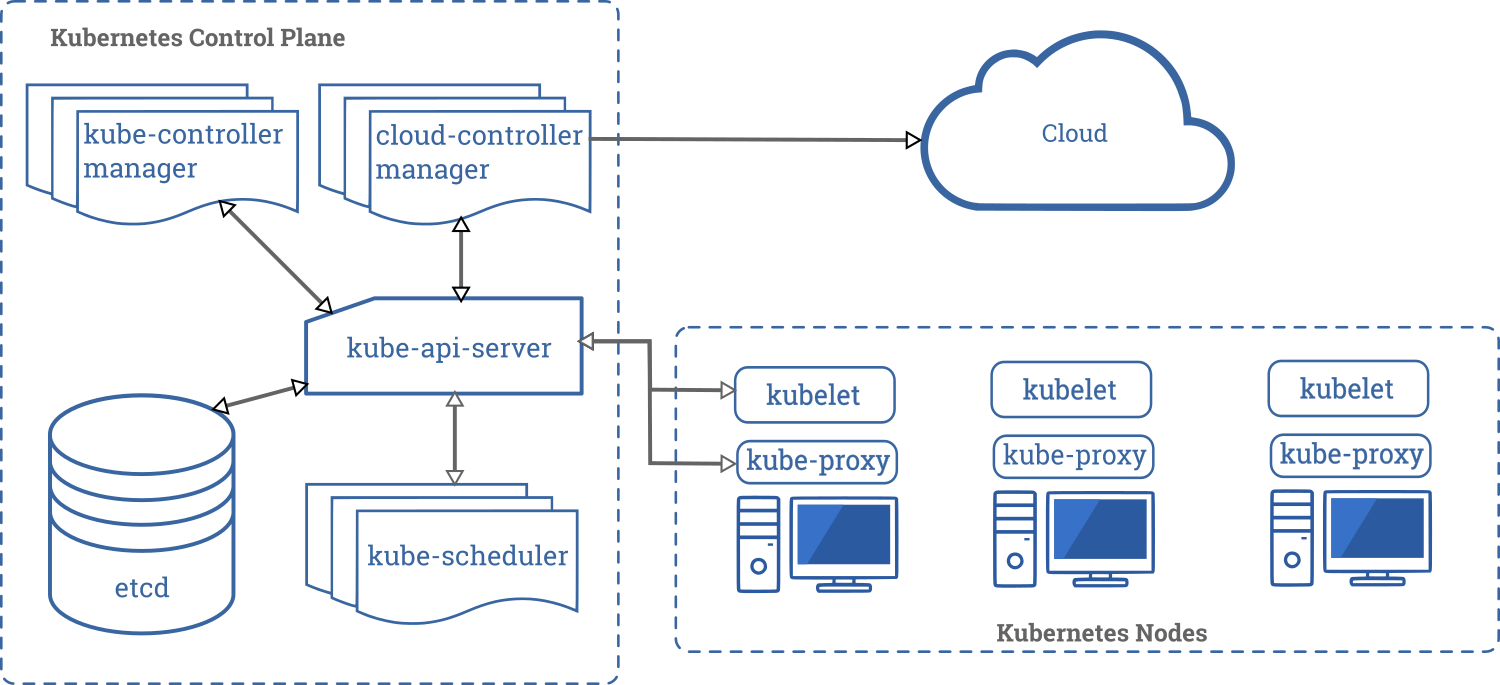
\includegraphics[width=1.0\textwidth]{./Figure/Kubernetes_Architettura.png}
 \caption{Architettura di Kubernetes}
 \label{fig:Architettura}
\end{figure}

\subsection{Kubernetes Control Plane}
Il Kubernetes Control Plane è il centro nevralgico delle operazioni del cluster. È costituito da una serie di componenti, in esecuzione all'interno del cluster, che hanno il compito di garantire l'integritá esecutiva del cluster, ad esempio, lo scheduling dei Worker Node e la gestione dei possibili failures dei Pod.
\begin{itemize}
    \item\textbf{kube-apiserver}
    kube-apiserver è il server API per il cluster Kubernetes. È il punto di contatto centrale a cui accedono tutti gli utenti, l'automazione e i componenti nel cluster Kubernetes. Il server API implementa un'API RESTful su HTTP, esegue tutte le operazioni API ed è responsabile dell'archiviazione degli oggetti API in un backend di archiviazione persistente. 
    \item\textbf{etcd}
    etcd è la componente di archiviazione principale di Kubernetes, etcd memorizza e replica tutti gli stati dei cluster Kubernetes. Il meccanismo di memorizzazione che adotta è di tipo chiave-valore ovvero ad ogni valore memorizzato viene associato una chiave che rappresenta il suo identificatore univoco. In questo modo il Control Plane è in grado di storicizzare gli stati del Cluster confrontando lo stato attuale con quello desiderato in modo di intervenire tempestivamente in caso di necessità.
    \item\textbf{kube-scheduler}
    kube-scheduler è la componente che consente al Control Plane lo scheduling dei Pod sui nodi. il kube-scheduler controlla i pod appena creati che non hanno un nodo assegnato, e dopo averlo identificato glielo assegna. 
    % DA RIVEDERE ✌️
    \item\textbf{kube-controller-manager} 
    Da un punto di vista logico, ogni controller è un processo separato, ma per ridurre la complessità, tutti i principali controller di Kubernetes vengono raggruppati in un unico container ed eseguiti in un singolo processo.
    Alcuni esempi di controller gestiti dal kube-controller-manager sono:
    Node Controller: Responsabile del monitoraggio dei nodi del cluster, e.g. della gestione delle azioni da eseguire quando un nodo diventa non disponibile.
    Replication Controller: Responsabile per il mantenimento del corretto numero di Pod per ogni ReplicaSet presente nel sistema
    Endpoints Controller: Popola gli oggetti Endpoints (cioè, mette in relazioni i Pods con i Services).
    Service Account e Token Controllers: Creano gli account di default e i token di accesso alle API per i nuovi namespaces.
    % DA RIVEDERE ✌️
    \item\textbf{cloud-controller-manager}
    Un componente della control plane di Kubernetes che aggiunge logiche di controllo specifiche per il cloud. Il cloud-controller-manager ti permette di collegare il tuo cluster con le API del cloud provider e separa le componenti che interagiscono con la piattaforma cloud dai componenti che interagiscono solamente col cluster.
    Il cloud-controller-manager esegue dei controller specifici del tuo cloud provider. Se hai una installazione Kubernetes on premises, o un ambiente di laboratorio nel tuo PC, il cluster non ha un cloud-controller-manager.
    Come nel kube-controller-manager, il cloud-controller-manager combina diversi control loop logicamente indipendenti in un singolo binario che puoi eseguire come un singolo processo. Tu puoi scalare orizzontalmente (eseguire più di una copia) per migliorare la responsività o per migliorare la tolleranza ai fallimenti.
    
    I seguenti controller hanno dipendenze verso implementazioni di specifici cloud provider:

    Node Controller: Per controllare se sul cloud provider i nodi che hanno smesso di rispondere sono stati cancellati
    Route Controller: Per configurare le network route nella sottostante infrastruttura cloud
    Service Controller: Per creare, aggiornare ed eliminare i load balancer del cloud provider

\end{itemize}